%\chapter{Construcción de supercondensadores}
Un supercondensador es construido simplemente haciendo un sándwich electrodo-separador-electrodo. El electrodo es una lámina del material activo, este puede estar depositado en un colector de corriente, o ser una lámina libre. Por otro lado, el separador es una membrana permeable al electrolito, como puede ser una membrana microporosa o papel filtro de celulosa, como primera aproximación se procede como en la figura \ref{fig:SC_process}.

\begin{figure}[h!]
	\centering
	\fbox{
		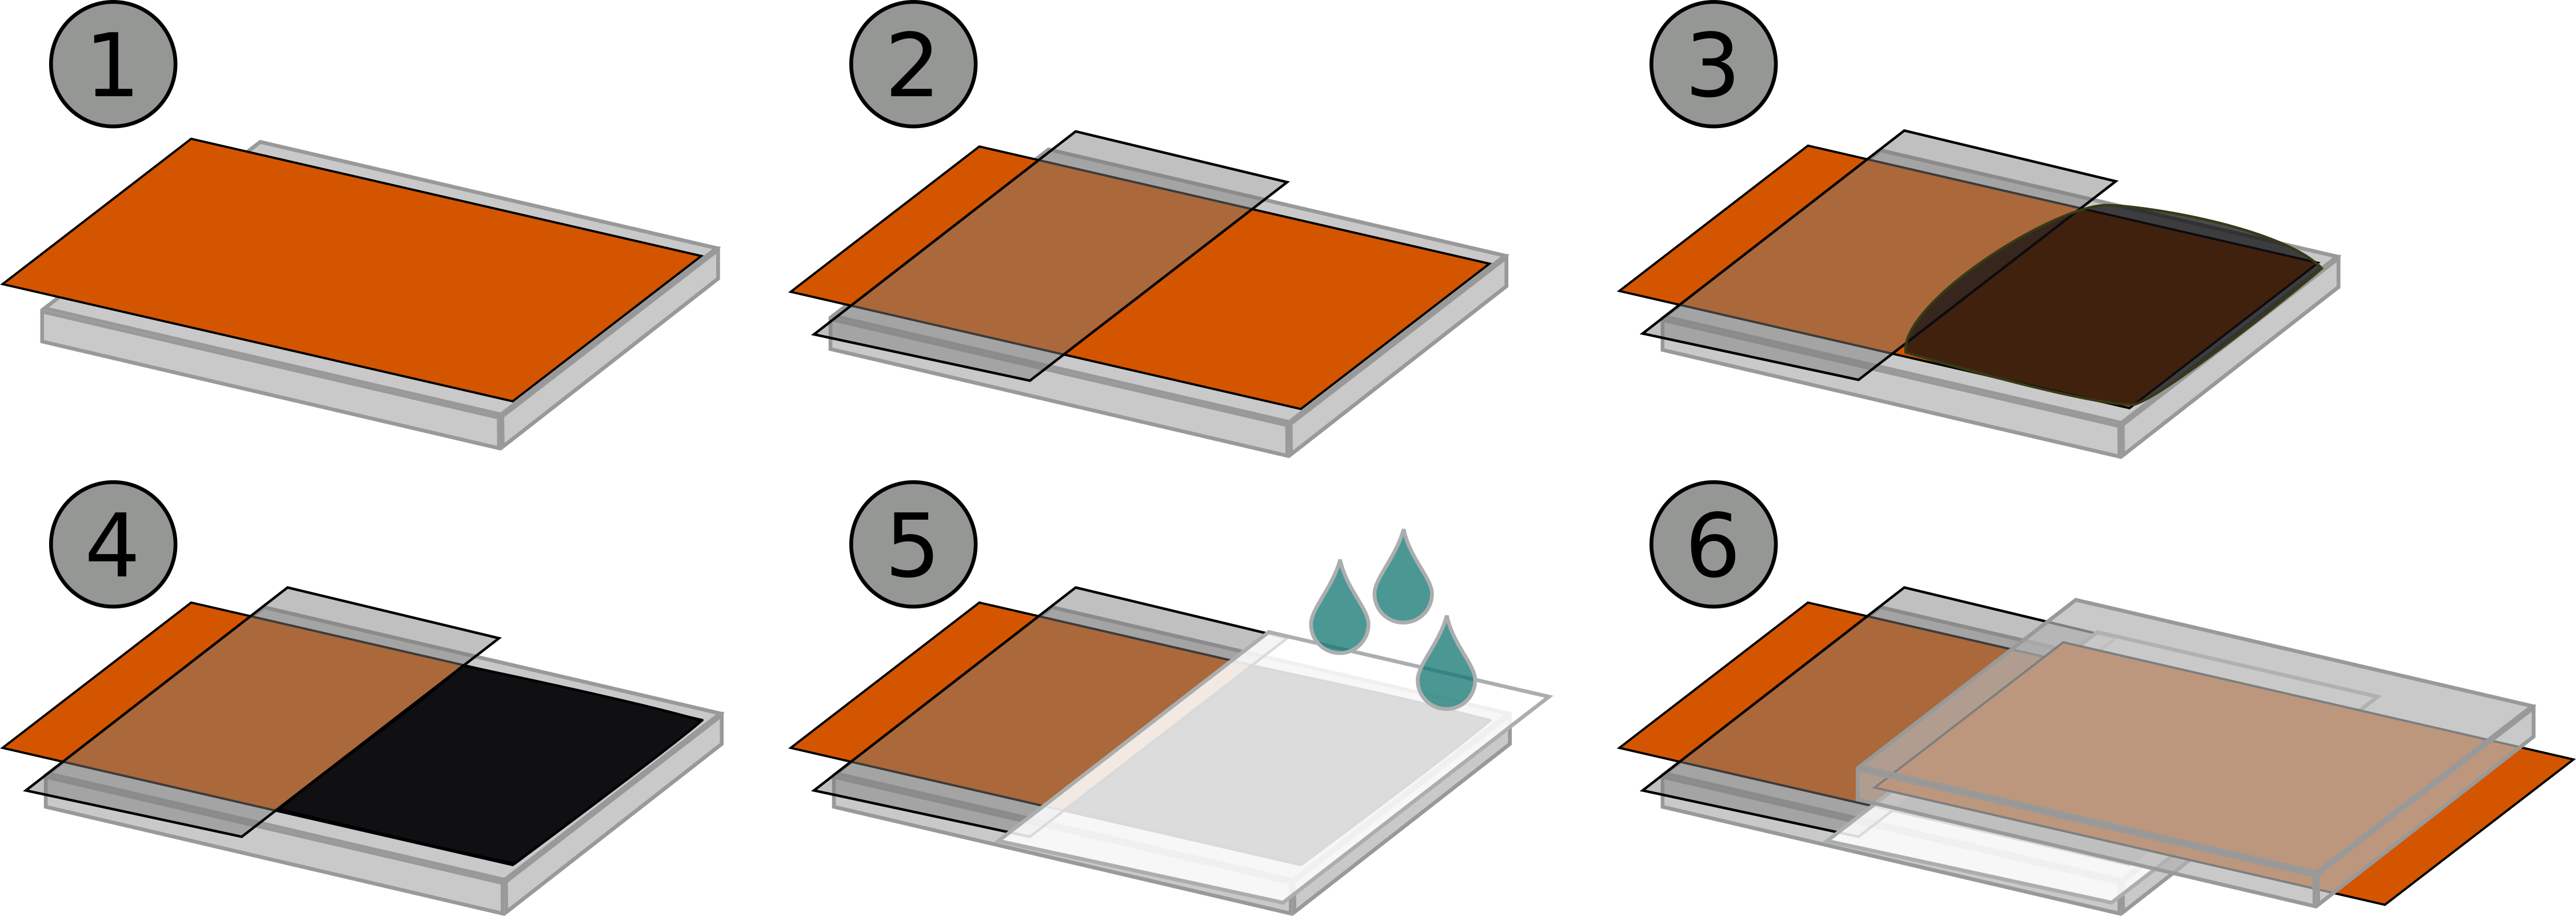
\includegraphics[width = 0.9\textwidth]{SC_process.png}
		}
	\caption{}
	\label{fig:SC_process}
\end{figure}

\section{Celda de pruebas de supercondensador}
La construcción de supercondensadores como se detalla anteriormente, presenta varios inconvenientes: (1) la deposición de material en los colectores de corriente no es homogénea, (2) el agua del electrolito se evapora rápidamente, (3) el cierre del dispositivo no es estable, y por consiguiente (4) la conexión a los terminales no es segura. Por estas razones, se diseña una celda que de pruebas que solucione estos problemas.
La celda diseñada y construida (ver figura \ref{fig:celda_de_pruebas_SC}) consta de dos colectores de corriente de acero inoxidable, entre los que se ubica el condensador como tal. Los colectores de corriente tienen sellos que impiden la fuga del electrolito o la evaporación del agua en él, permitiendo una operación estable en el tiempo. Los colectores de corriente se apoyan en bloques de acero que cierran la celda con pernos y permiten conectar los terminales del potenciostato a la celda de pruebas.

\begin{figure}[h!]
	\centering
	\fbox{
		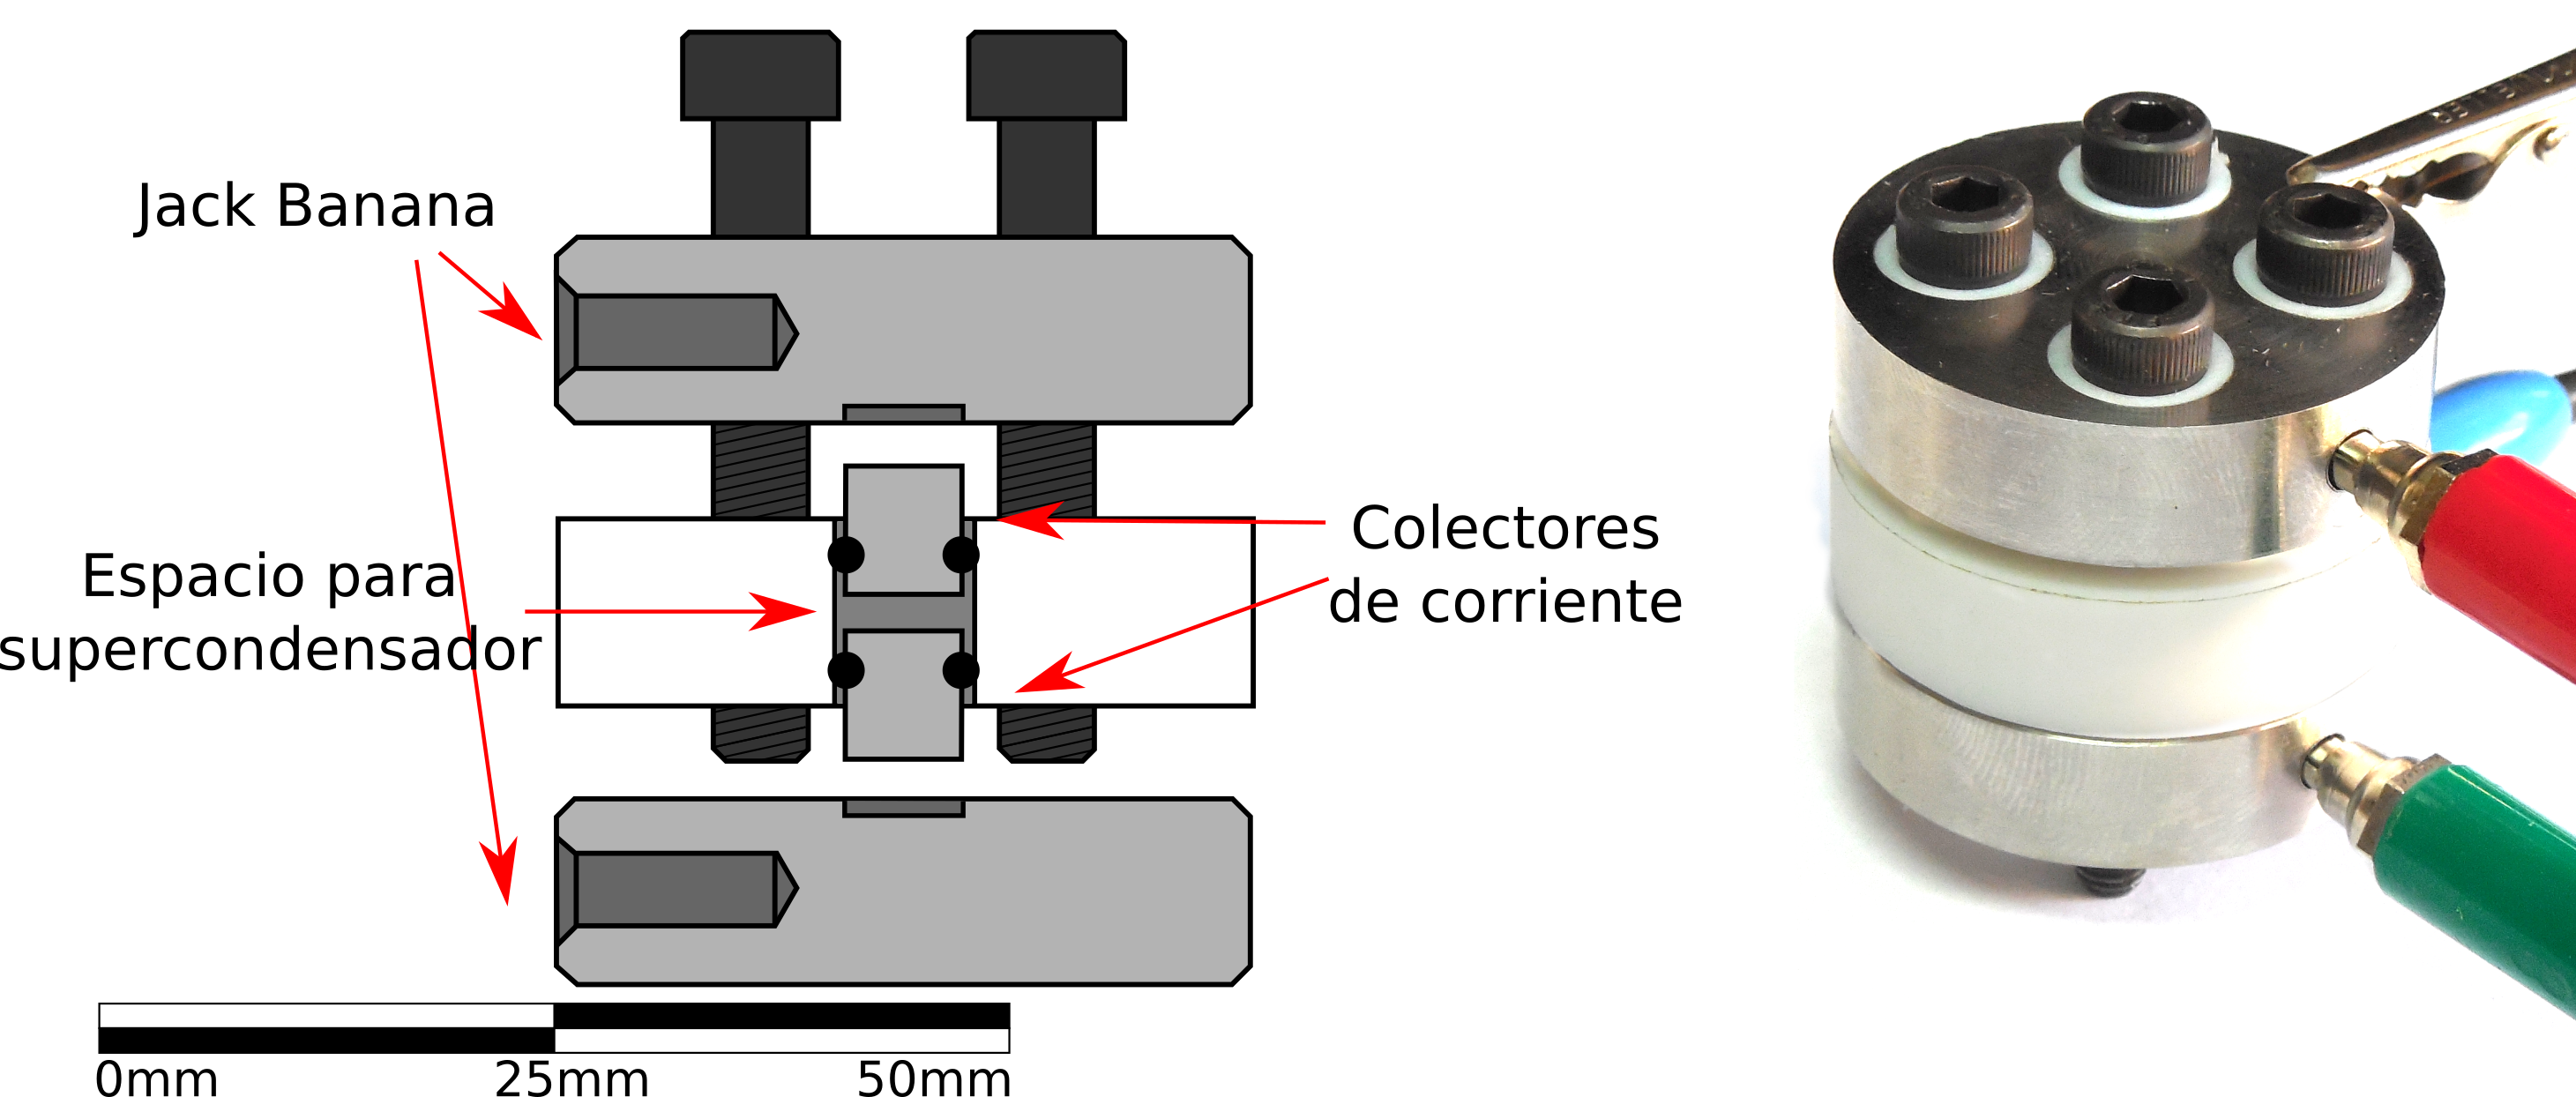
\includegraphics[width=0.8\textwidth]{cell3.png}
		}
	\caption{Izquierda: Vista longitudinal de la celda de pruebas, mostrando los componentes más importantes. Derecha: Fotografía de la celda armada y conectada al potenciostato.}
	\label{fig:celda_de_pruebas_SC}
\end{figure}

\section{Construcción de electrodos y preparación de electrolitos}
Los electrodos de rGO son fabricados mediante filtración por vacío. En este método de filtración, se dispersa el rGO en agua, la que se filtra por un filtro de celulosa en un embudo Büchner conectado a un kitasato y una bomba de vacío, el filtro con el material atrapado se deja secar a temperatura ambiente formando una lámina, la que es desprendida con facilidad del filtro de celulosa y luego recortada al tamaño apropiado para la celda de pruebas.

\begin{figure}
	\centering
	\fbox{
		\includegraphics[width=1.0\textwidth]{rgo_electrodes.png}
		}
	\caption{Electrodos utilizados en la celda de pruebas de supercondensador. De izquierda a derecha: Electro sin material depositado. Electrodo con material depositado mediante goteo (\emph{drop-casting}). Electrodo con material en forma de papel descentrado. Electrodo con material en forma de papel bien centrado soble el metal.}
	\label{fig:electrodes}
\end{figure}

\section{Resultados}
Los supercondensadores son sometidos a pruebas electroquímicas para estudiar su desempeño, estás pruebas incluyen: voltametría cíclica (CV), ciclos de carga y descarga a corriente constante, espectroscopía de impedancia electroquímica (EIS). Todas las mediciones electroquímicas son hechas con un potenciostato/galvanostato (Interface 5000E, Gamry).


\begin{figure}
	\centering
	\begin{subfigure}{0.3\textwidth}
		\begin{tikzpicture}[trim axis right,trim axis left]
		\begin{axis}
		[
		title=Voltametría Cíclica,
		domain=-0.8:0.8,
		ylabel={Corriente [A]},
		xlabel={Voltage [V]},
		cycle list name=exotic,
		no markers,
		]
		
		\addplot table {./Data/CV_CRGO300517_1/raw/sample1.txt};
		\addplot table {./Data/CV_CRGO300517_1/raw/sample2.txt};
		\addplot table {./Data/CV_CRGO300517_1/raw/sample3.txt};
		\addplot table {./Data/CV_CRGO300517_1/raw/sample4.txt};
		\addplot table {./Data/CV_CRGO300517_1/raw/sample5.txt};	
		\end{axis}
		\end{tikzpicture}
	\end{subfigure}\hfill
	\begin{subfigure}{0.3\textwidth}
		\begin{tikzpicture}[trim axis right,trim axis left]
		\begin{axis}
		[
		title=Voltametría Cíclica,
		domain=25:400,
		ylabel={Capacidad específica [F/g]},
		xlabel={Velocidad de barrido [mV/s]},
		cycle list name=exotic,
		]
		
		\addplot table {./Data/CV_CRGO300517_1/raw/capacitance.txt};	
		\end{axis}
		\end{tikzpicture}
	\end{subfigure}
	
	\begin{subfigure}{0.3\textwidth}
		\begin{tikzpicture}[trim axis right,trim axis left]
		\begin{axis}
		[
		title=Voltametría Cíclica,
		domain=-0.8:0.8,
		ylabel={Corriente [A]},
		xlabel={Voltage [V]},
		cycle list name=exotic,
		no markers,
		]
		
		\addplot table {./Data/CV_CRGO300517_2/raw/sample1.txt};
		\addplot table {./Data/CV_CRGO300517_2/raw/sample2.txt};
		\addplot table {./Data/CV_CRGO300517_2/raw/sample3.txt};
		\addplot table {./Data/CV_CRGO300517_2/raw/sample4.txt};
		\addplot table {./Data/CV_CRGO300517_2/raw/sample5.txt};	
		\end{axis}
		\end{tikzpicture}
	\end{subfigure}\hfill
	\begin{subfigure}{0.3\textwidth}
		\begin{tikzpicture}[trim axis right,trim axis left]
		\begin{axis}
		[
		title=Voltametría Cíclica,
		domain=25:400,
		ylabel={Capacidad específica [F/g]},
		xlabel={Velocidad de barrido [mV/s]},
		cycle list name=exotic,
		]
		
		\addplot table {./Data/CV_CRGO300517_2/raw/capacitance.txt};	
		\end{axis}
		\end{tikzpicture}
	\end{subfigure}
	\caption{pgfplots test 2.}
\end{figure}

\begin{figure}
	\centering
	\begin{subfigure}{0.3\textwidth}
		\begin{tikzpicture}[trim axis right,trim axis left]
			\begin{axis}
				[
				title=Voltametría Cíclica,
				domain=-0.8:0.8,
				ylabel={Corriente [A]},
				xlabel={Voltage [V]},
				cycle list name=exotic,
				no markers,
				]
				
				\addplot table {./Data/CV_CRGO300517_2/raw/sample1.txt};
				\addplot table {./Data/CV_CRGO300517_2/raw/sample2.txt};
				\addplot table {./Data/CV_CRGO300517_2/raw/sample3.txt};
				\addplot table {./Data/CV_CRGO300517_2/raw/sample4.txt};
				\addplot table {./Data/CV_CRGO300517_2/raw/sample5.txt};	
			\end{axis}
		\end{tikzpicture}
	\end{subfigure}\hfill
	\begin{subfigure}{0.3\textwidth}
		\begin{tikzpicture}[trim axis right,trim axis left]
			\begin{axis}
				[
				title=Voltametría Cíclica,
				domain=25:400,
				ylabel={Capacidad específica [F/g]},
				xlabel={Velocidad de barrido [mV/s]},
				cycle list name=exotic,
				]
				
				\addplot table {./Data/CV_CRGO300517_2/raw/capacitance.txt};	
			\end{axis}
		\end{tikzpicture}
	\end{subfigure}
	\caption{pgfplots test 2.}
\end{figure}
